% Template for ICASSP-2015 paper; to be used with:
%          spconf.sty  - ICASSP/ICIP LaTeX style file, and
%          IEEEbib.bst - IEEE bibliography style file.
% --------------------------------------------------------------------------
\documentclass{article}
\usepackage{spconf,amsmath,graphicx,qtree,tabularx}
\usepackage{times}
\usepackage{latexsym}
\usepackage{graphicx}
\usepackage{listings}

\usepackage{tikz}
\usetikzlibrary{positioning}
%% Example definitions.
% --------------------
\def\x{{\mathbf x}}
\def\L{{\cal L}}

% Title.
% ------
\title{Investigation of random forests in the synthesis of Mathematical Content}
%
% Single address.
% ---------------
\name{Sai Sirisha Rallabandi, Sai Krishna Rallabandi, Naina Teertha, Suryakanth V Gangashetty}
\address{International Institute of Information Technology, Hyderabad}
%
% For example:
% ------------
%\address{School\\
%	Department\\
%	Address}
%
% Two addresses (uncomment and modify for two-address case).
% ----------------------------------------------------------
%\twoauthors
%  {A. Author-one, B. Author-two\sthanks{Thanks to XYZ agency for funding.}}
%	{School A-B\\
%	Department A-B\\
%	Address A-B}
%  {C. Author-three, D. Author-four\sthanks{The fourth author performed the work
%	while at ...}}
%	{School C-D\\
%	Department C-D\\
%	Address C-D}
%
\begin{document}
%\ninept
\maketitle

\begin{abstract}

In this paper we investigate the use of  the Decision Trees for Unit Selection Speech Synthesis for appropriate synthesis of the mathematical equations.There also statistical methods for speech synthesis but The biggest drawback with statistical parametric synthesis versus unit-selection synthesis is the quality of synthesized speech

As a part of submission we have also shown that Unit selection speech synthesis performs better than the statistical speech synthesis by RNN.

\end{abstract}

\section{Introduction}
\label{sec:intro}

Text to speech (TTS) systems hold promise as an information access tool for literate and illiterate including visually challenged. Current TTS systems can convert a typical text into a natural sounding speech. However, auditory rendering of mathematical content, specifically equation reading is not a trivial task. Mathematical equations have to be read so that appropriate bracketing such as parentheses, superscripts and subscripts are conveyed to the listener in an accurate way. We have addressed this issue in our previous work[] by proposing four different techniques to render the equations in audio. We extended the framework further for other statistical data in [] where we applied the techniques for rendering pie and bar charts as well. In this paper, we extend the framework to the statistical parametric synthesis domain by incorporating random forests as the acoustic models. 
 

 

In this paper, we show that concatenative speech synthesis gives better results than the statistical synthesis. In Section 2, we briefly describe about the Significance of the work and in Section 3 we describe the scope of the work followed by  Present work, experimental results and conclusion.
\section{Significance of the work}
Mathematical content comprise of different types of visual cues to convey their semantic meaning. Some of these visual cues are superscripts, subscripts, parentheses,etc.  To effectively resolve such ambiguities and identify such demarcations need to be mapped to their auditory equivalent. Mathematics, in its visual form, gives the reader a very high level granularity in perceiving the equation. Mathematical equations, when presented in audio must be able to match the advantage in granularity provided in visual representation of mathematics.  In [], we first performed an experiment to measure the effectiveness of mathematical equations synthesised  using a traditional TTS system. We then analysed the acoustic cues which human-beings employ while speaking the mathematical content to (visually challenged) listeners and then proposed four techniques which render the observed patterns in a text-to- speech system.  

\section{Scope of the work}
We have used statistical parametric synthesis to render the equations in our previous work. Typical data size is 5 hours. As that much data is not available for equations ( the data is typically of half hour - one hour), the voices used were either Arctic [arctic database] or built from audiobooks [kishore sir thesis], both when text was available and when it was not [tejas journal].  However, as the original recordings were not aimed at rendering mathematical equations, the prosody was not natural. The voices built using only half hour of data had too much muffledness and buzziness due to parameter data sparsity[zavier lattorre paper]. Recently, Random forests have been proposed for acoustic modeling [ alan blak interspeech]. It was observed in that paper that RFs were performing well for low data. Therefore, we investigate the performance of the RFs for the task of equation rendering. More precisely, we seek answers to the questions: Can RFs be used to build voice using less data as in the case of eqn rendering? Can we improve the performance by using a selection criterion to select the trees as opposed to Random selection? 

\section{Proposed techniques}
\label{sec:techniques}
With the advent of languages like MathML, it is possible to programatically identify different attributes and visual cues of a mathematical expression. This possibility can in turn be leveraged to make some modifications  while generating speech for mathematical content.  We propose four techniques that could enhance the way mathematical content is rendered in audio.

\begin{figure}[h]
\label{fig:res}

\begin{minipage}[b]{1.0\linewidth}
  \centering
  
  \centerline{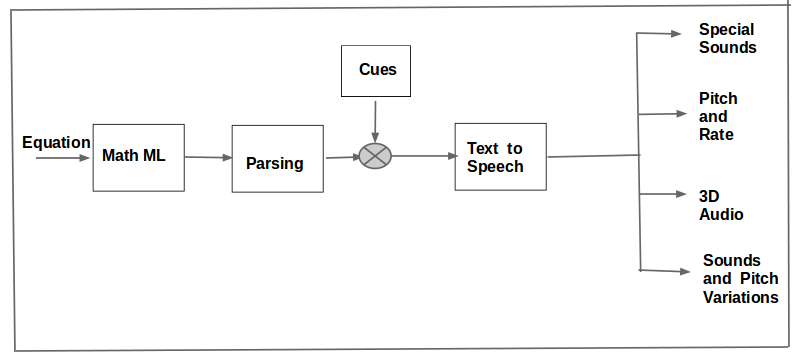
\includegraphics[width=8.5cm]{block}}
 
%  \vspace{2.0cm}
  \centerline{Fig: Overall framework for the proposed techniques}\medskip
\end{minipage}
\end{figure}

An example depicting the workflow of the entire algorithm is shown in the Figure 1. For the sake of illustration, a simple expression , $(X+Y)^{4-2} $ was taken :

\begin{figure}[t]
\caption{Example Synthesis using a simple expression}
\vspace{8pt}
\resizebox{8cm}{12cm}{
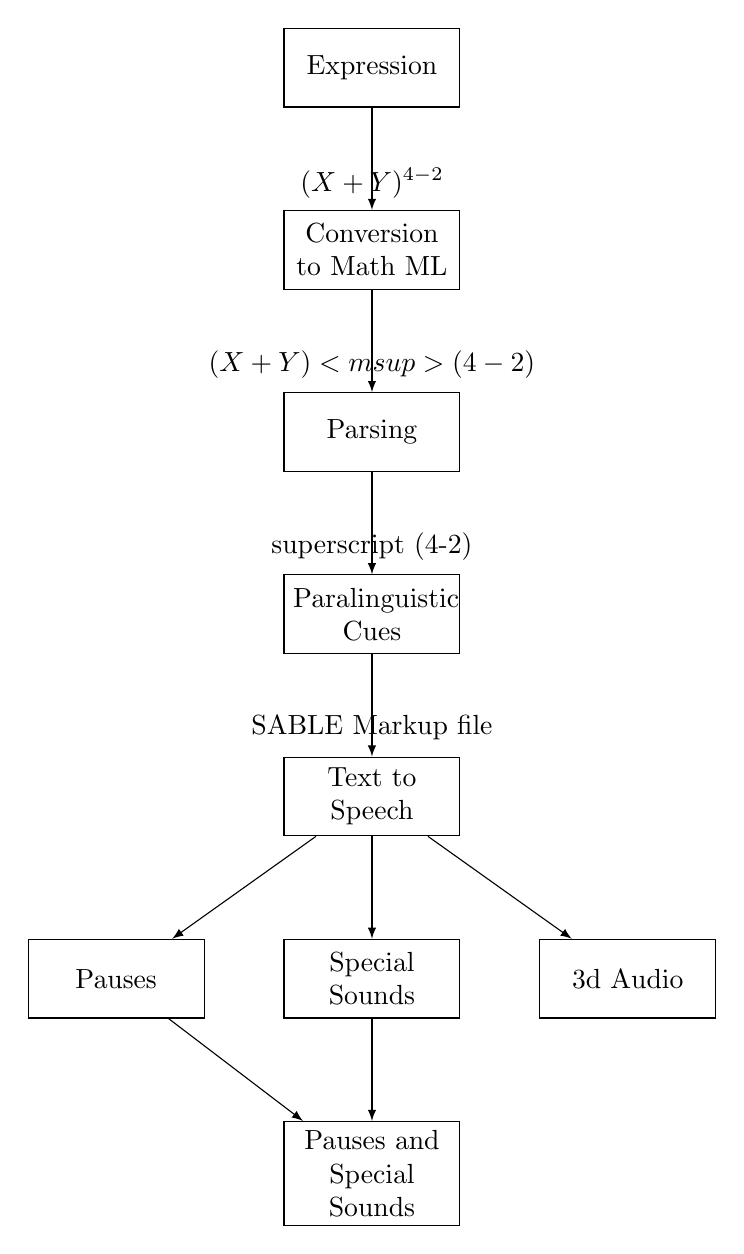
\begin{tikzpicture}[
node distance=1.3cm and 1cm,
ar/.style={->,>=latex},
mynode/.style={
  draw,
  text width=2cm,
  minimum height=1cm,
  align=center
  }
]
\node[mynode] (expression) { Expression};
\node[mynode,below=of expression] (MML) {Conversion to Math ML};
\node[mynode,below=of MML] (Parse) {Parsing};
\node[mynode,below=of Parse] (Cue) {Paralinguistic Cues};
\node[mynode,below =of Cue] (TTS) {Text to Speech};
\node[mynode,below left=of TTS] (1) { Pauses};
\node[mynode,below=of TTS] (2) {Special Sounds};
\node[mynode,below right=of TTS] (3) { 3d Audio};
\node[mynode,below right =of 1] (4) {Pauses and Special Sounds};

\draw[ar] 
  (expression) -- node[below] {$(X+Y)^{4-2} $} (MML);

\draw[ar] 
  (MML) -- node[below] { $(X+Y) <msup> {(4-2)}$} (Parse);

\draw[ar] 
  (Parse) -- node[below] {superscript (4-2)} (Cue);

\draw[ar] 
  (Cue) -- node[below] {SABLE Markup file} (TTS);

\draw[ar] 
  (TTS) -- node[below left] {} (1);

\draw[ar] 
  (TTS) -- node[below ] {} (2);

\draw[ar] 
  (TTS) -- node[below right ] {} (3);

\draw[ar] 
  (1) -- node[below  ] {} (4);

\draw[ar] 
  (2) -- node[below  ] {} (4);

\end{tikzpicture}
}
\end{figure}

The Equation was first converted into the Math Markup Language format. We chose "Presentation" Markup style to represent the equations.  
It is then text processed to identify and segregate the different terms occurring in the equation. The following terms have been segregated.

\begin{itemize}
\item Subscripts and superscripts 
\item Fractions
\item Square root terms
\item Overscripts and underscript
\end{itemize}

The MathML representation is processed to convert it into natural language and the acoustic cues such as pauses, intonation are incorporated to generate a file in the SABLE markup language \cite{sproat1998sable}. 
%Here's an example of the SABLE file:
The SABLE file is input to the speech synthesis system which generates the audio form of the equation with specified pauses and intonation.







\section { Decision Trees }
\label{sec:decision trees}
Decision tree learning uses a decision tree as a predictive model which maps observations about an item to conclusions about the item's target value. It is one of the predictive modelling approaches used in statistics, data mining and machine learning. Tree models where the target variable can take a finite set of values are called classification trees. In these tree structures, leaves represent class labels and branches represent conjunctions of features that lead to those class labels. Decision trees where the target variable can take continuous values (typically real numbers) are called regression trees. CART is powerful because it can deal with incomplete data, multiple types of features  both in input features and predicted features, and the trees it produces often contain rules which are humanly readable.

 CART analysis consists of four basic steps.The first step consists of tree building, during which a tree is built using recursive splitting of nodes. Each resulting node is assigned a predicted class, based on the distribution of classes in the learning dataset which would occur in that node and the decision cost matrix. The assignment of a predicted class to each node occurs whether or not that node is subsequently split into child nodes. The second step consists of stopping the tree building process. At this point a “maximal” tree has been produced, which probably greatly overfits the information contained within the learning dataset.  The third step consists of tree “pruning,” which results in the creation of a sequence of simpler and simpler trees, through the cutting off of increasingly important nodes.The fourth step consists of optimal tree selection, during which the tree which fits the information in the learning dataset,but does not overfit the information, is selected from among the sequence of pruned trees.
   
 Two applications of statistically-generated decision trees to problems in speech synthesis are described: (1) End of sentence detection: A decision tree is generated to decide when a period in text corresponds to the end of a declarative sentence (and not an abbreviation). The result is 99.8 percentage correct classification on the Brown corpus. (2) Segment duration modelling in speech synthesis: 1500 utterances from a single speaker were used to a build a decision tree that predicts segment durations based on features such as lexical position, stress, and phonetic context. The result is prediction with residuals with a 23 millisecond standard deviation and synthesis that compares favorably with current hand-generated duration rules.







\section{Conclusion}

 Through this work, we have  presented a new approach to math accessibility by making effective use of speech cues by concatenative speech synthesis. We have also shown that concatenative speech synthesis performs better than that of the statistical parametric synthesis.
. We tabulated a series of experiments performed with  concatenative synthesis using decision trees and statistical synthesis.This work shall be further extended...............

\end{document}




